\section{Results}\label{sec:analysis}

\begin{table}[t]
\begin{small}
\begin{tabular}{| c | p{1.6in} |}\hline
\textbf{Parameter} & \textbf{Definition}	\\\hline
Traffic Demand per Subscriber& \(\frac{\text{total bytes transferred in 
measurement int.}}{\text{number of contributing subscribers}}\)	\\
Peak Demand & Daily maximum number of bytes transferred in any 15-minute
interval \\ 
Prime-Time Ratio 	& \( \frac{ \text{avg usage in peak (prime-time) 
hour}}{ \text{avg usage in off-peak hour}}\) 		\\
Peak Ratio 		& \(\frac{\text{95\%-ile of daily traffic 
demand}}{\text{mean of daily traffic demand}}\)	\\\hline
\end{tabular}
\end{small}
\caption{Evaluation Metrics.}
\label{tab:eval-criteria}
\end{table}

\paragraph{Metrics}
Table~\ref{tab:eval-criteria} shows the metrics that we use to evaluate
how user demand responds to service-tier upgrades. The \emph{traffic
  demand} for a subscriber is defined as the total bytes transferred, in
upstream or downstream, during a single sample measurement (15 minutes).
We use traffic demand to calculate the total demand per hour, and the
average and 95th percentile peak demand over a day. To compare the total
traffic of the control and treatment groups, we scale to a thousand
subscribers wherever applicable (Table~\ref{tab:data-stats}).  We
define \emph{prime time} as 8:00 p.m. to 12:00 a.m., when Internet usage
tends to be highest.  Indeed, we
observed that the total daily traffic consistently falls within 90th percentile
during this four-hour period. We define the \emph{prime-time ratio} as
the ratio of traffic during an average prime-time hour, to the average
hourly traffic outside the prime-time hour.  This ratio conveys the
disparity between demand during the prime-time and the rest of the day.
The rest of this section explores the effects of a service-tier upgrade
on user traffic demand in the context of these metrics.

\subsection{Traffic Demand Per Subscriber}\label{subsec:behavior}

\begin{figure}[t]
\begin{minipage}{1\linewidth}
\centering
%
\begin{subfigure}[b]{.99\linewidth}
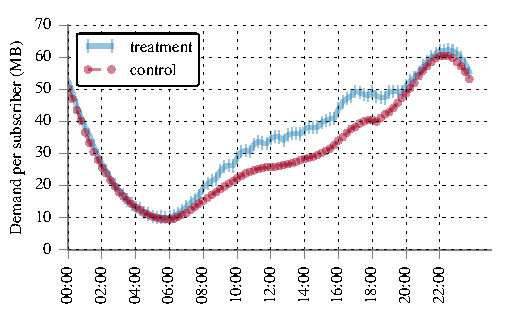
\includegraphics[width=\linewidth]{figures/weekday_demand_mean.pdf}
               \caption{Weekday traffic demand\label{fig:weekday-daily-usage}}
\end{subfigure}
%
\begin{subfigure}[b]{.99\linewidth}
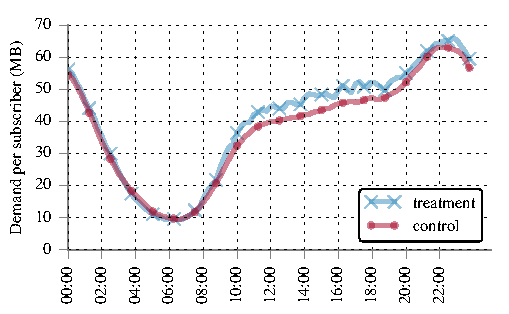
\includegraphics[width=\linewidth]{figures/weekend_demand_mean.pdf}
               \caption{Weekend traffic demand\label{fig:weekend-daily-usage}}
\end{subfigure}
%
\end{minipage}
\caption{Average subscriber demand (bytes every 15-minutes)}
\label{fig:traffic-demand-timeseries}
\end{figure}

Figure \ref{fig:traffic-demand-timeseries} shows the downlink traffic demand (bytes)
of an average subscriber over a 15-minute measurement period in a week.
We observe that subscriber behavior differs
significantly on weekdays and weekends. On weekdays, traffic demand 
increases monotonically from morning until prime-time in the evening. On 
weekends, there is a sharp rise in demand in the early morning period. Then, the
demand plateaus until the next sharp rise during the evening prime-time hours.
Previous reports indicate that the aggregate traffic volume for US fixed access
link providers usually troughs during mid-afternoon hours (between 2:00 PM -- 6:00 PM)
~\cite{sandvine20141h}. We do not observe such a trough in the subscriber 
demand in our dataset.

\begin{figure}[t]
\begin{minipage}{1\linewidth}
\centering
%
\begin{subfigure}[b]{1\linewidth}
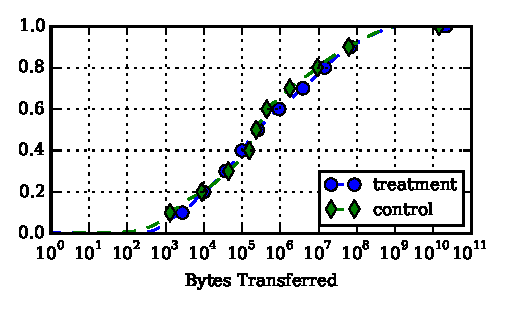
\includegraphics[width=\linewidth]{figures/cdf-all-bytes.pdf}
               \caption{Overall traffic demand for all subscribers at all times\label{fig:CDF-data-rate}}
\end{subfigure}
% maybe should be mean per day?
%
\begin{subfigure}[b]{1\linewidth}
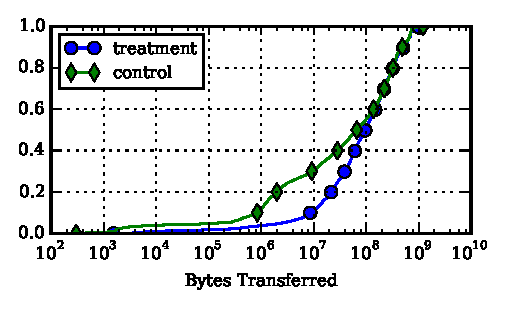
\includegraphics[width=\linewidth]{figures/cdf-per-device-perc95.pdf}
               \caption{Peak (95\%) traffic demand per subscriber\label{fig:CDF-data-rate-perc95}}
\end{subfigure}
%
\end{minipage}
\caption{Traffic demand (bytes every 15-minutes) for \control{} and \treatment{}\label{fig:traffic-demand-cdf}}
\end{figure}

Figure \ref{fig:CDF-data-rate} shows the distribution of the
all bytes transferred in the \treatment{} and \control{} set
over the three months of the dataset. Figure \ref{fig:CDF-data-rate-perc95}
plots the distribution of the peak (95th percentile) demand of the
subscriber over the three months of the dataset. The highest peak
demand achieved by subscribers in the \control{} and \treatment{}
groups were 10 GB in 15-mins. The median peak demand was 80 MB and
100 MB respectively.

We observe that although the overall series are similar, the peak demand of subscribers
is higher in the \treatment{} set. We expected the largest difference
in demands would be in the subscribers who have the heaviest demand already.
But unexpectedly, the lowest demanding 50\% of the subscribers in
\treatment{} have a much higher demand than the lowest demanding 50\% of \control{}.
We confirm that the both groups have similar median demands over each day. However
the daily peak demand is higher for the lowest demanding subscribers in
 \treatment{}, as compared to the lowest demanding subscribers in \control{}.

\begin{figure}[t]
\centering
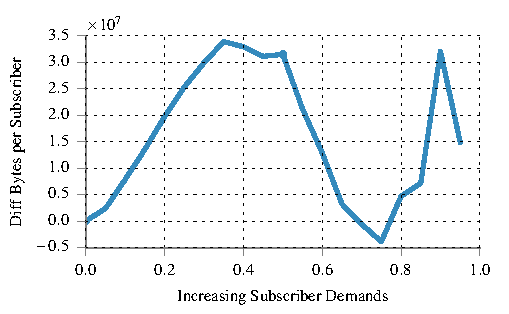
\includegraphics[width=\linewidth]{figures/diff_perc95_bytes_subsc-overall.pdf}
               \caption{Difference between \treatment{} and \control{}
               in peak (95\%) traffic demand\label{fig:diff-perc95}}
\end{figure}

We plot the distribution of the difference in peak subscriber demands for
the lowest to highest demanding subscribers in both groups (Figure~\ref{fig:diff-perc95}).
We see that the peak demand for the lowest demanding 70\% of the households of
the \treatment{} group is higher than the peak demand of the lowest demanding bottom-most
70\% of the \control{} group. These subscribers have a peak demand less than 200 MB.
For 20\% of the subscribers in the \control{} group with peak demands between 10 -- 70 MB,
the equivalent 20\% of the \treatment{} group has peak demands increased by 30 MB.

Under 15\% of subscribers in the \treatment{} group with peak demands more than 200 MB 
peak demands similar, or lower than the equivalent 15\% of subscribers in the \control{}
group, that has a lower capacity. The highest demanding subscribers in the \treatment{}
(beyond 800 MB peak demand) have demands 15 -- 30 MB more than the equivalent 15\% of 
the \control{} group. For the upstream, the \treatment{} group consistently has
a 2 MB higher peak traffic demand every 15 minutes as compared to the \control{} group
(except for the top 10\% users in the \treatment{} set who had a higher peak).

\begin{figure}[t]
\centering
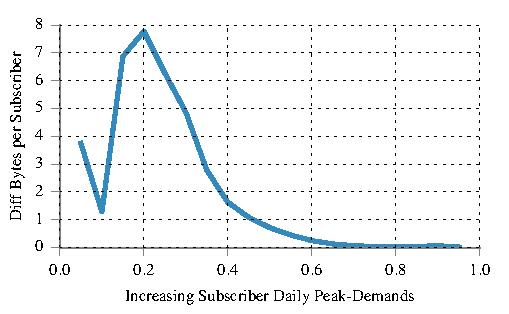
\includegraphics[width=\linewidth]{figures/diff_perc95_bytes_subsc-daily-normalized.pdf}
               \caption{Ratio of the difference between \treatment{} and \control{}
               in the daily peak traffic demand to the daily peak of the \control\label{fig:daily-ratio-perc95}}
\end{figure}

On investigating further, we observed that a similar percentage of 
subscribers with low peak demand in \control{} had a higher peak demand in \treatment{}.
40\% of the subscribers with lowest daily peak demands in the \treatment{} still
had more than double the traffic demand of the equivalent 40\% in the \control{} group.
(see Figure~\ref{fig:daily-ratio-perc95})

the 
There is negligible change in the daily peak 
demand for users who have high demands, and a large increase for users with a low demand.
Furthermore, we observe this affect is also present in the uplink.
There could be many reasons for this increase in demand, such as short
term activities (short videos or web browsing) 
that have a slightly higher traffic demand. Studying the applications 
responsible for such behavioral changes in traffic demand is out of the
scope of this paper and we leave it to future work.

\subsection{Prime-Time Ratio} \label{subsec:primetime}

The daily diurnal nature of Internet traffic demand requires that ISP providers 
design networks capable of handling load at the times when heaviest usage is 
observed. Such heavy demand is usually observed during prime time hours in the 
evening, when many subscribers heavily consume real-time entertainment traffic
(video) (seen as primarily responsible for high usage during these hours). The FCC defines 
Prime-Time as the local time from 7:00 PM to 11:00 PM.
\cite{fcc2014measuring-broadband}. To measure the concentration of network usage
during prime-time, we use Sandvine's definition of the \emph{Prime-Time 
ratio}: the ratio of the average traffic demand during prime-time hours to the average 
traffic demand in non-prime-time hours.\cite{sandvine20141h, sandvine20142h}.

We measure the prime-time ratio of the \control{} and \treatment{} group
for each contiguous four hour period in our datasets to find the evening hours with
the largest prime-time ratio. We observed that in our dataset,
the prime time ratio consistently peaks at 8:00 PM -- 12:00 AM for both
datasets.

%\begin{figure}[t]
%\begin{minipage}{1\linewidth}
%\centering
%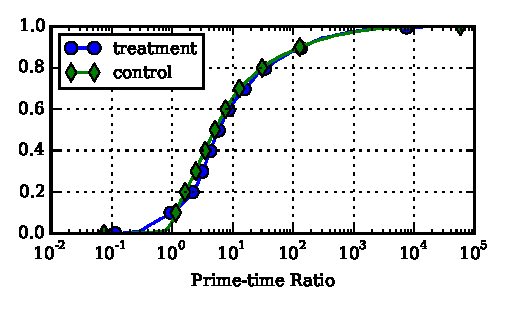
\includegraphics[width=1\linewidth]{figures/prime-time-ratio-per-device-cdf-MEAN.pdf}
%\caption{Prime-Time Ratio\label{fig:cdf-prime-time-ratio}}
%\end{minipage}
%\end{figure}

%\begin{subfigure}[]{.32\linewidth}
%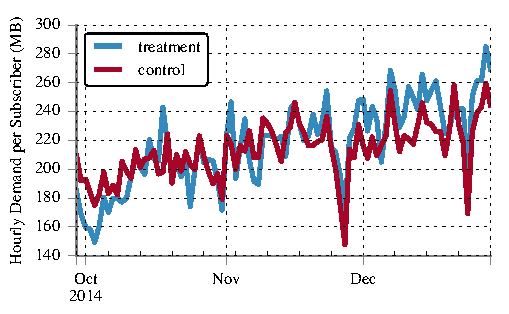
\includegraphics[width=1\linewidth]{figures/primetime_usage_per_day_per_subs.pdf}
%\caption{\label{fig:pt}}
%\end{subfigure}

%\begin{subfigure}[b]{.32\linewidth}
%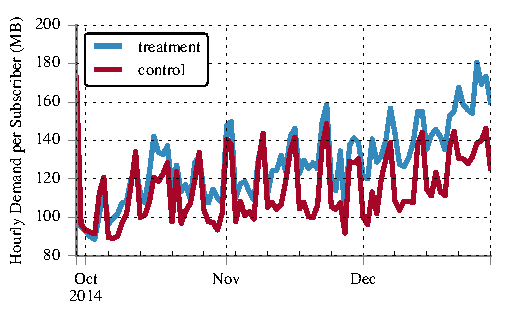
\includegraphics[width=1\linewidth]{figures/nonprimetime_usage_per_day_per_subs.pdf}
%\caption{\label{fig:non-pt}}
%\end{subfigure}


We observed that the hourly downlink traffic per 1000 subscribers between 8:00 PM -- 12:00 AM is 
209.5 GB for \treatment{}, and 205.1 GB for \control{}. However, during an average hour
outside of prime time, the traffic per 1000 subscribers is 122.3 GB for the higher tier
and 108.5 GB for the lower tier. This difference in demand during hours outside of the
daily prime-time is also apparant from the weekly usage patterns in Figure~\ref{fig:traffic-demand-timeseries}.

\begin{table}[t]
\begin{tabular}{| cc | c |c | }\hline
  &                    & Weekday         & Weekends \\\hline
\multirow{2}{*}{\begin{tabular}[c]{@{}l@{}}Hourly Traffic in\\ Prime-Time\end{tabular}}
& treatment          & 233.12          & 246.93   \\
& control            & 225.40          & 238.15   \\\hline
\multirow{2}{*}{\begin{tabular}[c]{@{}l@{}}Hourly Traffic in\\ Non-Prime-Time\end{tabular}}
& treatment & 124.18 & 143.08    \\
& control   & 104.30  & 133.16  \\\hline
\multirow{2}{*}{\begin{tabular}[c]{@{}l@{}}Prime-Time Ratio\end{tabular}}
& treatment & \textbf{1.88} &  1.73 \\
& control  &  \textbf{2.16} &  1.79 \\\hline
\end{tabular}
\caption{Hourly Traffic Demand during in prime-time hours (MB)\label{prime-time-demand}}
\end{table}


We calculate the prime-time ratio per day for the 
datasets groups over weekends and weekdays, as shown in Table \ref{prime-time-demand}.
%in figure~\ref{fig:cdf-prime-time-ratio}. A comparison shows 
On weekends, the prime-time ratios for both groups are
1.73 and 1.79 respectively. On the weekdays, the prime-time ratio for \control{}
is much higher, 2.16, as compared to treatment, 1.88. The demand
during prime-time hours on the weekdays for \treatment{} is within 4\% of
the \control{} traffic, thus there is no substantial
change. In contrast, the demand in non-prime-time hours (outside 8:00 PM -- 12:00 PM)
is much higher in the \treatment{} group, especially on weekdays. 

By definitition, the prime-time ratio is measured using total traffic volume in a day.
For our dataset, the prime-time ratio for the \treatment and \control groups
were 1.70 and 1.93 respectively. However, not all subscribers contribute equally
to the traffic volume. We observed that the median prime-time ratio \emph{per subscriber}
is 3.39 for the \treatment{} group and 2.91 for the \control{} group. This indicates
that demand during prime-time per subscriber has increased, but the total
traffic volume during non-prime-time hours has also increased substantially. For
subscribers that have a larger aggregate demand during non-prime-time hours, the prime
time ratio will be less than one. We found 9\% of the \control{} group and 14\% of 
the treatment group showed this behavior. These subscribers may be small home-run businesses,
users who work at home, or just users who have unexpected usage behaviors. 6\% of the 
subscribers in both groups had a prime-time ratio over 100.

Thus the overall demand of subscribers in the \treatment{} may have decreased by 
total volume of traffic, however, it has increased on a per-subscriber basis.
This result indicates that individual subscribers that do not contribute substantially
to the traffic volume are the ones who have higher usage in prime-time as compared to their
lower tier counterparts.

%Latency and performance 
%are adversely affected during prime-time, causing bottlenecks at home, the last 
%mile, in
%transit, or at the content server. For example, the Sandvine Global
%Internet Phenomena Report \footnote{The Sandvine Reports ~\cite{sandvine20141h,
%sandvine20142h}are released bi-annually and
%contain a detailed analysis of aggregate Internet usage. They are also referred
%to in the FCC reports~\cite{fcc2015progress-report, fcc2014measuring-broadband,
%fcc2014progress-report}} showed that devices in the same household selected  
%Netflix's own CDN (OpenConnect) during off-peak hours, and third party CDNs 
%(with differing
%performance) during prime-time. This may happen because Netflix OpenConnect is
%over-utilized during prime time~\cite{sandvine20141h}.

\subsection{User Taxonomy based on Peak Ratio}
\label{subsec:peakratio}
% the ratio of the 90\%-ile to the median throughput per day.

\begin{figure}[ht!]
\begin{minipage}{0.90\linewidth}
\centering
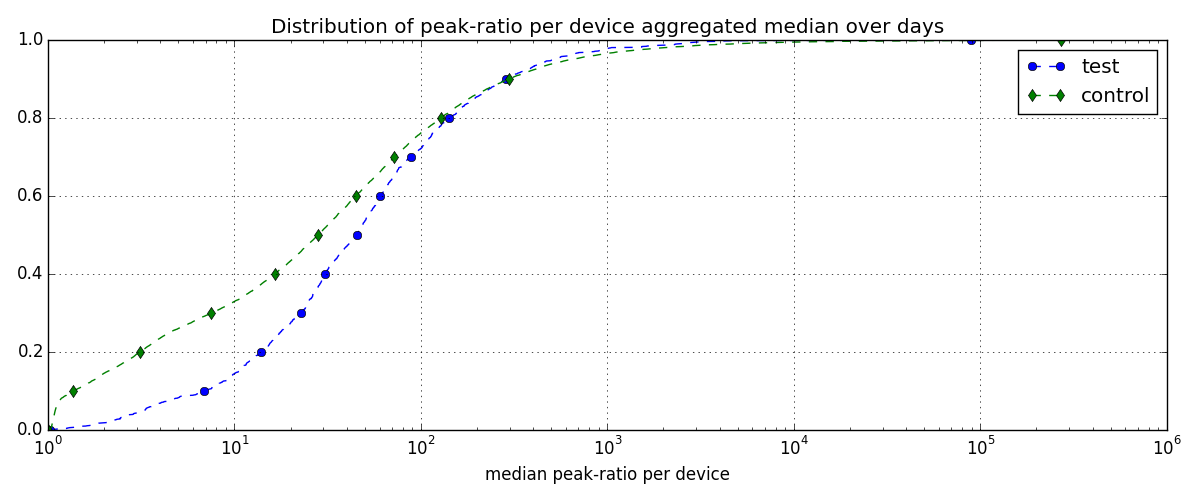
\includegraphics[width=1\linewidth]{figures/peakratio-CDF-devices-MEDIAN.png}
\caption{Median peak ratio per device showing that test set has higher daily ratio (50 times by median). Thus ISPs should condition their networks to 50 times the median usage for each user added in the worst case scenario.}
%http://sites.noise.gatech.edu/~sarthak/files/comcast/plots/full_dw/peakratio-CDF-devices-MEDIAN.png
\label{fig:CDF-peak-ratio-median}
\end{minipage}
\end{figure}

\paragraph{Peak Ratio: }To further characterize and compare the deviation of data rate for the \control and \test set, we examine \emph{peak-ratio} as defined in ~\ref{sec:methodology} 
Figure ~\ref{fig:CDF-peak-ratio-median} shows that the median peak-ratio for each device in the \test set is much larger than that of the \control set.
\todo{replace much larger with the exact number or percentage}.
\sg{Taken together} with our observations of a lower prime-time ratio of the \test set (section~\ref{subsec:primetime}) this implies that there are households in the \test set that achieve a peak-ratio $>$ 1, but not during the prime-time hour. We believe that these households might actually be small businesses or work-at-home users that peak during daytime hours instead of evening hours.

\begin{figure}[ht!]
\begin{minipage}{0.9\linewidth}
\centering
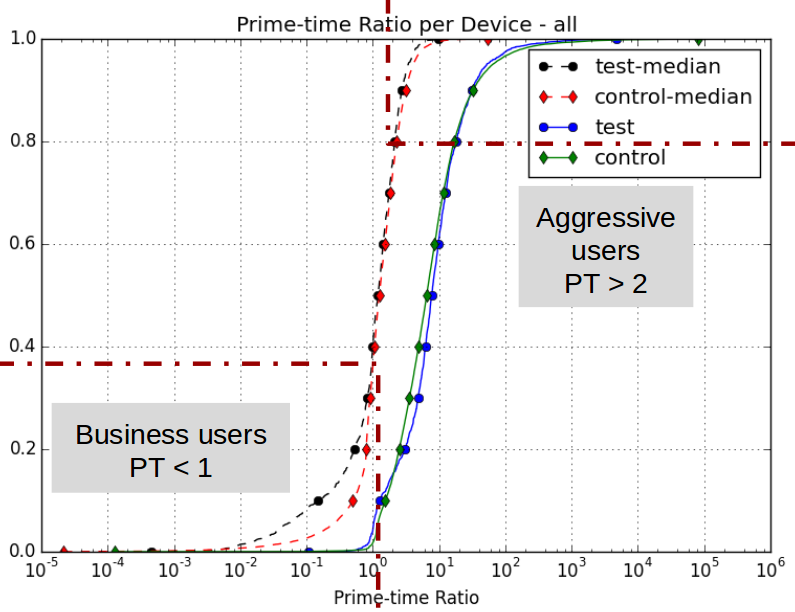
\includegraphics[width=0.9\linewidth]{figures/cdf-prime-time-ratio[replace].png}
\caption{(old) Prime Time ratio + usage can be used to divide users into four sets: aggressive all time + non aggressive all time, aggressive peak time, aggressive non-peak time (business hours). 30\% PT $<$ 1: possibly businesses with normal work-hours . 20\% PT $>$ 2: aggressive prime-time streamers}
%http://riverside.noise.gatech.edu:8083/separated/full/cdf-prime-time-ratio-per-device.png\\
%http://riverside.noise.gatech.edu:8083/plots/full_dw/prime-time-ratio-per-device-cdf-ALL.png
\label{fig:CDF-prime-time-ratio}
\end{minipage}
\end{figure}

The median peak-ratio per device itself shows a large range, from 1 to 10e6 (figure~\ref{fig:CDF-peak-ratio-median}), and the maximum peak-ratio per device was an order higher. Clearly there are some households that have a very even usage throughout the day (low peak ratio), and others that are extremely aggressive only at certain times (high peak ratio). We plot this segregation in figure ~\ref{fig:CDF-prime-time-ratio}.

\todo{EVERYTHING BELOW THIS IS TODO AND TODISCUSS}

\paragraph{User Taxonomy:} The Sandvine reports present a taxonomy of users based on their contribution to real-time entertainment traffic. We incorporate a similar definition based on contribution to data traffic, along with our observations of utilization, to present a taxonomy of the users in our dataset. One category of users is the non-utilizers, i.e., non-aggressive low bandwidth users, that contribute less than SOME THRESHOLD PERCENTILE to the daily data transferred \sg{these the ISP can ignore, also they probably don't need this tier as their utilization from the previous section must be super low}. The second category is of users contributing most aggressively to the data at the ISP \sg{these users will probably gobble up a higher capacity link if given a chance - they're the ones who effect all our graphs.. Need to check this claim}. We further subdivide this high utilizing subcategory based on differing prime-time ratio and peak-ratios follows... \todo{need to think and analyze this further: technical definition to do the analysis}
\begin{itemize}
\item Aggressive All-Time: Users having a low peak-ratio due to a lower variance. Is also expected to have a low prime-time ratio.
\item Aggressive Prime-Time: The usual streamer with a high prime-time ratio and a high peak ratio.
\item Aggressive Non-Prime-Time: Possibly a business user with a low prime-time ratio  but a high peak ratio
\end{itemize}

% other results:
%big difference (2 x median ratio) in per device per day ratios of 90%ile:median.
%weird shape again for values < ratio 100
%big difference in this ratio per day, and it is consistent across all individual sets + months.
%very large for Dec, slightly smaller for Nov
%interestingly, at higher ratios control is slightly > test. This means that certain devices in control set have a huge std (ratio) in a day as compared to test set which has a lower “max” ratio.

\todo{ TO PLOT :}
\begin{itemize}
\itemsep0em
\item peak ratio cdf vs no of devices
\item peak ratio cdf vs time of day where peak occurred
\item no of devices cdf vs time of day where peak occurred
\end{itemize}

Based on differing usage profiles within the same high tier bandwidth, we suggest that the FCC adopt multiple benchmarks based on usage characteristics to better characterize broadband availability, deployment, and adoption in the US. Such multiple benchmarks can be the minimum broadband speed required per user based on the kind of traffic expected during a day. ISPs can also offer these users better plans based on hour-of-the-day or usage caps to encourage more off-peak usage. These users probably don't cause latency spikes in PT.


We recommend multiple standards...


% PUT RESULTS TABLE HERE

%\subsection{Aggressive Subscribers}\label{subsec:prevalence}

\begin{figure}[ht]
\begin{minipage}{\linewidth}
\centering
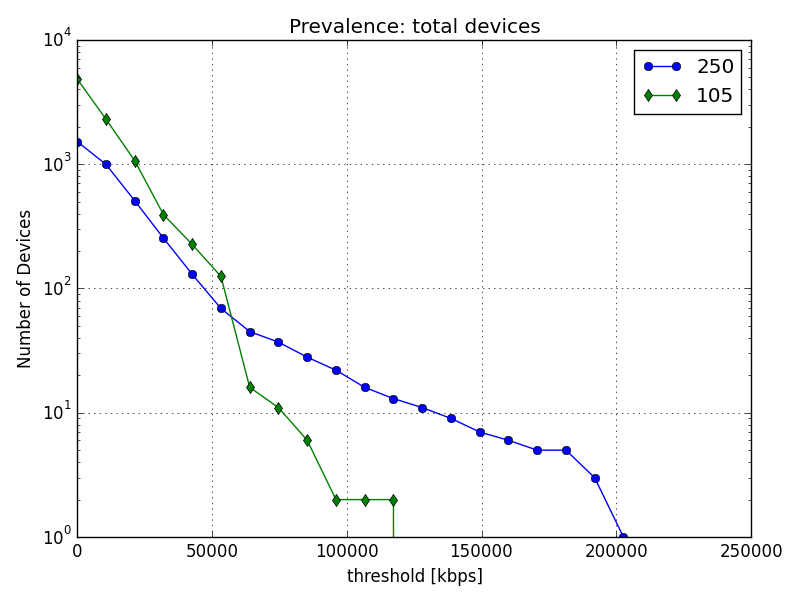
\includegraphics[width=\linewidth]{figures/prevalence.png}
\caption{User prevalence as threshold increases.}
\label{fig:prevalence}
\end{minipage}
\end{figure}

Outliers. Prevalence.
While the general behavior did not change, still 11 users maxed out traffic.
For example (explain the fig)